% Template LaTeX source file for homework problem solutions.
% Alan T. Sherman (9/9/98)
% Updated: Greg King (2014)

% Running LaTeX
%
% Name this file FOO.tex
% latex FOO
% latex FOO   
%    (You have to run latex twice to get the cross references correct.
%     Running latex creates a file FOO.dvi 
%     You can view dvi files with the program xdvi )
% xdvi FOO.dvi &
%
% lpr -d FOO.dvi
%    (To print the dvi file.   Be sure to use the "-d" print option,
%     and be sure your printer can handle dvi files (not all printers can).
%     Do NOT print with "lpr FOO.dvi", which will print tens of pages
%     of unreadable dvi source code. Printing a postscript (ps) file
%     is usually more reliable, as explained below.)
%
% dvips FOO.dvi
%    (To create a postscript file named FOO.ps 
%     which you can view with the program ghostview )
% ghostview FOO.ps &
% lpr FOO.ps
%    (To print the ps file.)

%%%%%%%%%%%%%%%%%%%%%%%%%%%%%%%%%%%%%%%%%%%%%%%%%%%%%%%%%%%%%%%%%%%%%%

\documentclass[letter,12pt]{article}

\RequirePackage{amsmath}
\RequirePackage{amsmath,amssymb,amsthm}
\RequirePackage{tikz}
\usepackage{listings}
\usepackage{color}
\usepackage{textcomp}
\usepackage{graphicx}
\usepackage{hyperref}
\usepackage{afterpage}

\renewcommand{\lstlistlistingname}{Code Listings} 
\renewcommand{\lstlistingname}{Code Listing} 
\definecolor{gray}{gray}{0.5} 
\definecolor{key}{rgb}{0,0.5,0} 
\lstnewenvironment{python}[1][]{ 
\lstset{
language=python,
basicstyle=\ttfamily\small,
otherkeywords={1, 2, 3, 4, 5, 6, 7, 8 ,9 , 0, -, =, +, [, ], (, ), \{, \}, :, *, !},
keywordstyle=\color{blue},
stringstyle=\color{red},
showstringspaces=false,
emph={class, pass, in, for, while, if, is, elif, else, not, and, or,
def, print, exec, break, continue, return},
emphstyle=\color{black}\bfseries,
emph={[2]True, False, None, self},
emphstyle=[2]\color{key},
emph={[3]from, import, as},
emphstyle=[3]\color{blue},
upquote=true,
morecomment=[s]{"""}{"""},
commentstyle=\color{gray}\slshape,
frame=tb,
rulesepcolor=\color{blue},#1
}}{}


\usetikzlibrary{calc}
\RequirePackage{tkz-euclide}
\usetkzobj{all}
%\usepackage{minted}
%\usepackage{fontspec}
%\setsansfont{Calibri}
%\setmonofont{Consolas}
%    \begin{minted}[mathescape,
%                   linenos,
%                   numbersep=5pt,
%                   gobble=2,
%                   frame=lines,
%                   framesep=2mm]{csharp}
%      string title = "This is a Unicode π in the sky"
%      /*
%      Defined as $\pi=\lim_{n\to\infty}\frac{P_n}{d}$ where $P$ is the perimeter
%      of an $n$-sided regular polygon circumscribing a
%      circle of diameter $d$.
%      */
%      const double pi = 3.1415926535
%    \end{minted}


%\usepackage[utf8]{inputenc}
%
%% Default fixed font does not support bold face
%\DeclareFixedFont{\ttb}{T1}{txtt}{bx}{n}{12} % for bold
%\DeclareFixedFont{\ttm}{T1}{txtt}{m}{n}{12}  % for normal
%
%% Custom colors
%\usepackage{color}
%\definecolor{deepblue}{rgb}{0,0,0.5}
%\definecolor{deepred}{rgb}{0.6,0,0}
%\definecolor{deepgreen}{rgb}{0,0.5,0}
%
%\usepackage{listings}
%
%% Python style for highlighting
%\newcommand\pythonstyle{\lstset{
%language=Python,
%basicstyle=\ttm,
%otherkeywords={self},             % Add keywords here
%keywordstyle=\ttb\color{deepblue},
%emph={MyClass,__init__},          % Custom highlighting
%emphstyle=\ttb\color{deepred},    % Custom highlighting style
%stringstyle=\color{deepgreen},
%frame=tb,                         % Any extra options here
%showstringspaces=false            % 
%}}
%
%
%% Python environment
%\lstnewenvironment{python}[1][]
%{
%\pythonstyle
%\lstset{#1}
%}
%{}
%
%% Python for external files
%\newcommand\pythonexternal[2][]{{
%\pythonstyle
%\lstinputlisting[#1]{#2}}}
%
%% Python for inline
%\newcommand\pythoninline[1]{{\pythonstyle\lstinline!#1!}}
%
%\begin{document}
%
%\section{``In-text'' listing highlighting}
%
%\begin{python}
%class MyClass(Yourclass):
%    def __init__(self, my, yours):
%        bla = '5 1 2 3 4'
%        print bla
%\end{python}
%
%\section{External listing highlighting}
%
%\pythonexternal{demo.py}
%
%\section{Inline highlighting}
%
%Definition \pythoninline{class MyClass} means \dots
%
%\end{document}
%    \begin{minted}{python}
%    def boring(args = None):
%    pass
%    \end{minted}

% Set the margins
%
\setlength{\textheight}{8.5in}
\setlength{\headheight}{.25in}
\setlength{\headsep}{.25in}
\setlength{\topmargin}{0in}
\setlength{\textwidth}{6.75in}
\setlength{\oddsidemargin}{0in}
\setlength{\evensidemargin}{0in}


%%%%%%%%%%%%%%%%%%%%%%%%%%%%%%%%%%%%%%%%%%%%%%%%%%%%%%%%%%%%%%%%%%%%%%%
% Macros

% Math Macros.  It would be better to use the AMS LaTeX package,
% including the Bbb fonts, but I'm showing how to get by with the most
% primitive version of LaTeX.  I follow the naming convention to begin
% user-defined macro and variable names with the prefix "my" to make it
% easier to distiguish user-defined macros from LaTeX commands.
%
\newcommand{\myN}{\hbox{N\hspace*{-.9em}I\hspace*{.4em}}}
\newcommand{\myZ}{\hbox{Z}^+}
\newcommand{\myR}{\hbox{R}}

\newcommand{\myfunction}[3]
{${#1} : {#2} \rightarrow {#3}$ }

\newcommand{\myzrfunction}[1]
{\myfunction{#1}{{\myZ}}{{\myR}}}


% Formating Macros
%

\newcommand{\myheader}[4]
{\vspace*{-0.5in}
\noindent
{#1} \hfill {#3}

\noindent
{#2} \hfill {#4}

\noindent
\rule[8pt]{\textwidth}{1pt}

\vspace{1ex} 
}  % end \myheader 

\newcommand{\myalgsheader}[0]
{\myheader{Stanford University, Department of Computer Science}
{Computer Science 224D}{Spring 2016}{Section 1}}

% Running head (goes at top of each page, beginning with page 2.
% Must precede by \pagestyle{myheadings}.
\newcommand{\myrunninghead}[2]
{\markright{{\it {#1}, {#2}}}}

\newcommand{\myrunningalgshead}[2]
{\myrunninghead{Computer Science 224D}{{#1}}}

\newcommand{\myrunninghwhead}[2]
{\myrunningalgshead{Solution to Assignment {#1}, Problem {#2}}}

\newcommand{\mytitle}[1]
{\begin{center}
{\large {\bf {#1}}}
\end{center}}

\newcommand{\myhwtitle}[3]
{\begin{center}
{\large {\bf Solution to Assignment {#1}, Problem {#2}}}\\
\medskip
{\it {#3}} % Name goes here
\end{center}}

\newcommand{\myhwintro}[3]
{\begin{center}
{\large {\bf Assignment {#1}, Problem {#2}}}\\
\medskip
{\it {#3}} % Name goes here
\end{center}}

\newcommand{\mysection}[1]
{\noindent {\bf {#1}}}

\newcommand{\solutionsAuthor}{Gregory King}
%%%%%% Begin document with header and title %%%%%%%%%%%%%%%%%%%%%%%%%
\begin{document}

\myalgsheader
%\myhwintro{2}{1 (Tensorflow Softmax)}{~}

\pagestyle{myheadings}
\thispagestyle{plain}
\setcounter{page}{1}
\myhwtitle{1}{1(a)}{\solutionsAuthor}

\bigskip
%Assn#1:
%1.29, 1.42, 1.43
%%%%% Begin Solution %%%%%%%%%%%%%%%%%%%%%%%%%%%%%%%%%%%%%%%%%%%%%%%%%%%

\noindent {\bf Softmax} Prove that softmax (denoted $\textrm{softmax}({\bf x})$)
is invariant to a constant offset in the input, that is, for any input vector
$\bf x$ and any constant $c$,
\begin{equation}
\textrm{softmax}({\bf x}) = \textrm{softmax}({\bf x} + c),
\end{equation}
where $({\bf x} + c)$ means adding the constant $c$ to every dimension of ${\bf x}$.

{\bf Note}: In practice, we make use of this property and choose $c = -\textrm{max}_{i}({\bf x_i})$, when computing $\textrm{softmax}$ probabilities for numerical stability (i.e. subtracting the maximum element from all elements of ${\bf x}$).\vspace{5mm}

\noindent\rule{\textwidth}{0.4pt}\vspace{5mm}

\noindent Starting from the definition of softmax,
\begin{equation}
\textrm{softmax}({\bf x})_{i} = \frac{e^{x_{i}}}{\sum_{j=1}{e^{x_{j}}}}
\end{equation}
it follows, the linear shift, ${\bf x} + c$, yields the following (for the $i$ element):
\begin{align}
\textrm{softmax}({\bf x} + c)_{i} & = \frac{e^{(x_{i} + c)}}{\sum_{j=1}{e^{(x_{j} + c)}}}\\
                                                 & = \frac{e^{c}}{e^{c}}\frac{e^{(x_{i})}}{\sum_{j=1}{e^{(x_{j})}}}\\
                                                 & = \textrm{softmax}({\bf x})_{i}
\end{align}
since this is true for an arbitary $i$, it follows immediately that the linear shift has no affect on the softmax probabilities.


%\sum_{j=1}{\exp{x_{j}}

% The vector addition diagram is drawn in Figure~\ref{solution figure:question 1.29}.
% Careful measurement gives $\vec{D}$ is around 144~m, $41^{\circ}$ south of west (scale is 1 grid point:50 m).
% \begin{figure}[!h!b]
% \begin{center}
% \begin{tikzpicture}
%   \draw[step=.5cm,gray,very thin](-2.,-2.) grid (2., 2.);
%   \draw[->,black,thick] (-2.,0) -- (2.,0) coordinate (x axis);
%   \draw[->,black,thick] (0,-2.) -- (0,2.) coordinate (y axis);
%   \coordinate (A) at (0,0);%start at orgin
%   \coordinate (B) at (-1.8,0);%go west 180 m
%   \coordinate (C) at (-0.315,-1.485);% go east 210 cos (315*) = 148.5m, go south 148.5m
%   \coordinate (D) at (1.085, 0.94);%go north 280 sin (60*) = 242.5 m, go east 280 sin(60*) = 140m
%   \draw[->,black,very thick] (A) -- node[above=2pt] {$\vec{A}$} (B);
%   \draw[->,black,very thick] (B) -- node[left=2pt] {$\vec{B}$}  (C);
%   \draw[->,black,very thick] (C) -- node[right=2pt] {$\vec{C}$} (D);
%   \draw[->,black,dashed, very thick] (D) -- node[above=2pt] {$\vec{D}$} (A);
% \end{tikzpicture}
% \end{center}\caption{Vector Diagram for (1.29)\label{solution figure:question 1.29}}
% \end{figure}

%% First page break
%%   Note: "myheadings" is a LaTeX keyword; it is not a user-defined entity.
%%
\clearpage
\pagestyle{myheadings}
\myrunninghwhead{1}{1 (Softmax)}

\myhwtitle{1}{1(b)}{\solutionsAuthor}

\bigskip

\noindent Given an input matrix of \texttt{N}-rows and \texttt{d}-columns, compute the softmax prediction for each row.
Write your implementation in \texttt{q1\_softmax.py}. You may test by executing python \texttt{q1\_softmax.py}.\\

\noindent \textbf{Note:} The provided tests are not exhaustive. Later parts of the assignment will reference this code so it is
important to have a correct implementation. Your implementation should also be efficient and vectorized
whenever possible. A non-vectorized implementation will not receive full credit!\vspace{5mm}

\noindent\rule{\textwidth}{0.4pt}
\begin{python}
import numpy as np

def softmax(x):
    c = np.max(x, axis=x.ndim - 1, keepdims=True)
    #for numerical stability
    y = np.sum(np.exp(x - c), axis=x.ndim - 1, keepdims=True)
    x = np.exp(x - c)/y
    return x
\end{python}
\clearpage

\myrunninghwhead{1}{2 (Neural Networks)}

\myhwtitle{1}{2(a)}{\solutionsAuthor}

\bigskip

\noindent Derive the gradients of the sigmoid function and show that it can be rewritten as a function of the
function value (i.e. in some expression where only $\sigma(x)$, but not $x$, is present). Assume that the input
$x$ is a scalar for this question.\vspace{5mm}

\noindent\rule{\textwidth}{0.4pt}\vspace{5mm}

\noindent Denote the sigmoid function as $\sigma(z)$,
\begin{equation}
\sigma(z) = \frac{1}{1 + e^{-z}}.
\end{equation}
It follows, using the chain rule (and noting that $e^{-z}= 1/\sigma(z) -1$),
\begin{align*}
\sigma^{\prime}(z)   &= \frac{-1}{(1+e^{-z})^{2}}\times(-e^{-z})\\
                                 &= \sigma^{2}(z)\left(\frac{1}{\sigma(z)} - 1 \right)\\
                                 &= \sigma(z) - \sigma^{2}(z)\\
                                 &= \sigma(z)(1 - \sigma(z))
\end{align*}

\clearpage

\myhwtitle{1}{2(b)}{\solutionsAuthor}
\bigskip

\noindent Derive the gradient with regard to the inputs of a softmax function when cross entropy loss is used for
evaluation, i.e. find the gradients with respect to the softmax input vector $\theta$, when the prediction is
made by $\hat{y} = \textrm{softmax}(\theta)$. Remember the cross entropy function is
\begin{equation}
\textrm{CE}({\bf y},{\bf\hat{y}}) = -\sum_{i}{y_{i}\log{\hat{y_{i}}}}
\end{equation}
where $y$ is the one-hot label vector, and $\hat{y}$ is the predicted probability vector for all classes. \vspace{2mm}\\
\noindent {\bf Hint}: you might want to consider the fact many elements of $y$ are zeros, and assume that only the $k$-th dimension
of $y$ is one.\vspace{5mm}

\noindent\rule{\textwidth}{0.4pt}\vspace{5mm}
Starting with, cross entropy,
\begin{equation}
\textrm{CE}({\bf y},{\bf\hat{y}}) = -\sum_{i}{y_{i}\log{\hat{y_{i}}}}
\end{equation}
We can derive the gradient of the cross-entropy function, using back propagation,
\begin{equation}
\frac{\partial(\textrm{CE})}{\partial{\hat{y}_{i}}} = -\frac{y_{j}}{\hat{y}_{i}}\label{eq:2b 1}
\end{equation}
Thus, 
\begin{align}
\frac{\partial(\textrm{CE})}{\partial{\theta_{k}}} = & \frac{\partial(\textrm{CE})}{\partial{\hat{y}_{i}}}\frac{\partial{\hat{y}_{i}}}{\partial{\theta_{k}}} \\
                                                                        = & -\frac{y_{j}}{\hat{y}_{i}}\frac{\partial{\hat{y}_{i}}}{\partial{\theta_{k}}}
\end{align}
Calculating the partial derivative of $\hat{y_{i}}$ (where $i=k$)
\begin{align}
\frac{\partial{\hat{y}_{i}}}{\partial{\theta_{i}}} = & \frac{\partial}{\partial{\theta_{i}}}\left( \frac{e^{\theta_{i}}}{\sum_{j=1}{e^{\theta_{j}}}}\right) \\
                                                                      = & \frac{e^{\theta_{i}}}{\sum_{j=1}{e^{\theta_{j}}}} - \left(\frac{e^{\theta_{i}}}{\sum_{j=1}{e^{\theta_{j}}}}\right)^{2} \\
                                                                      = & \hat{y}_{i}\cdot(1 - \hat{y}_{i})\label{eq:2b 2}
\end{align}
and (where $i\neq k$),
\begin{align}
\frac{\partial{\hat{y}_{i}}}{\partial{\theta_{k}}} = & \frac{\partial}{\partial{\theta_{k}}}\left( \frac{e^{\theta_{i}}}{\sum_{j=1}{e^{\theta_{j}}}}\right) \\
                                                                       = & - \left(\frac{e^{\theta_{i}}e^{\theta_{k}}}{\sum_{j=1}{e^{\theta_{j}}}}\right) \\
                                                                       = & - \hat{y}_{i}\hat{y}_{k}\label{eq:2b 3}
\end{align}
Combining Equations~\ref{eq:2b 1},~\ref{eq:2b 2},~\ref{eq:2b 3}, yields
\begin{equation}
\frac{\partial(\textrm{CE})}{\partial{\theta_{k}}} = \begin{cases}
-y_{j}(1 - \hat{y}_{k})&\text{ for }i=k \\
y_{j}\hat{y}_{k}&\text{ for }i\neq k
\end{cases}
\end{equation}
Requiring $y_{j}$ to be non-zero, imposes that the auxiliary condition, $k=j$ and $y_{j}=1$, hence it follows immediately,
\begin{equation}
\frac{\partial(\textrm{CE})}{\partial{\theta_{j}}} = \begin{cases}
(\hat{y}_{j} - 1)&\text{ for }i=j\label{eq:2b case 1} \\
\hat{y}_{j}&\text{ for }i\neq j
\end{cases}
\end{equation}
Which is equivalent to (with the substitution $y_{j}$ for $1$ in the first case of Equation \ref{eq:2b case 1}),
\begin{equation}
\frac{\partial(\textrm{CE})}{\partial{\boldsymbol\theta}} = \bf{\hat{y}} - \bf{y}
\end{equation}

\clearpage

\myhwtitle{1}{2(c)}{\solutionsAuthor}
\bigskip

\noindent Derive the gradients with respect to the inputs x to an one-hidden-layer neural network (that is, find
$\partial{J}/\partial{\bf x}$ where $J$ is the cost function for the neural network). The neural network employs sigmoid activation
function for the hidden layer, and softmax for the output layer. Assume the one-hot label vector is $y$,
and cross entropy cost is used. (feel free to use $\sigma^{\prime}(x)$ as the shorthand for sigmoid gradient, and feel free
to define any variables whenever you see fit). \vspace{5mm}\\
\def\layersep{2.5cm}
\begin{center}
\begin{tikzpicture}[shorten >=1pt,->,draw=black!50, node distance=\layersep]
    \tikzstyle{every pin edge}=[<-,shorten <=1pt]
    \tikzstyle{neuron}=[circle,fill=black!25,minimum size=17pt,inner sep=0pt]
    \tikzstyle{input neuron}=[neuron, fill=green!50];
    \tikzstyle{output neuron}=[neuron, fill=red!50];
    \tikzstyle{hidden neuron}=[neuron, fill=blue!50];
    \tikzstyle{annot} = [text width=4em, text centered]

    % Draw the input layer nodes
    \foreach \name / \y in {1,...,4}
    % This is the same as writing \foreach \name / \y in {1/1,2/2,3/3,4/4}
        \node[input neuron, pin=left:$x_{\y}$] (I-\name) at (0,-\y) {};

    % Draw the hidden layer nodes
    \foreach \name / \y in {1,...,5}
        \path[yshift=0.5cm]
            node[hidden neuron] (H-\name) at (\layersep,-\y cm) {};

    % Draw the output layer nodes
    \foreach \name / \y in {1,...,6}
        \path[yshift=0.75cm]
            node[output neuron] (O-\name) at (\layersep+\layersep,-\y cm) {};
%    % Draw the output layer node
%    \node[output neuron,pin={[pin edge={->}]right:Output}, right of=H-3] (O) {};

    % Connect every node in the input layer with every node in the
    % hidden layer.
    \foreach \source in {1,...,4}
        \foreach \dest in {1,...,5}
            \path (I-\source) edge (H-\dest);

%    % Connect every node in the hidden layer with the output layer
    \foreach \source in {1,...,5}
       \foreach \dest in {1,...,6}
        \path (H-\source) edge (O-\dest);

    % Annotate the layers
    \node[annot,above of=H-1, node distance=1cm] (hl) {$h$};
    \node[annot,left of=hl] {$x$};
    \node[annot,right of=hl] {$\hat{y}$};
\end{tikzpicture}
\end{center}
\noindent Recall that the forward propagation is as follows:
\begin{align}
{\bf h}         & = \textrm{sigmoid}({\bf x\textrm{W}_{1} + b_{1}}) \\
{\bf \hat{y}} & = \textrm{softmax}({\bf h\textrm{W}_{2} + b_{2}})
\end{align}
\noindent {\bf Note}: here we're assuming that the input vector (and thus the hidden variables and output probabilities)
is a row vector to be consistent with the programming part of the assignment. When we apply the sigmoid function to
a vector, we are applying it to each of the elements of the vector. $\bf{\textrm{W}}_i$ and $\bf{b}_{i}$ ($i\in\{1,2\}$) are
the weights and biases, respectively of the two layers.\vspace{5mm}

\noindent\rule{\textwidth}{0.4pt}\vspace{5mm}
In order to simplify the notation used to solve the problem, define the following terms:
\begin{align}
{\bf x}^{(2)} \equiv& \quad{\bf h} \\
{\bf z}_{i}     \equiv& \quad{\bf x^{(i)}\textrm{W}_{i} + b_{i}}
\end{align}
Now, to calculate $\partial{J}/\partial{\bf x^{1}}$, one can use the back propagation algorithm. Starting with the results from Question 2(b):
%\begin{equation}
%\frac{\partial J}{\partial{x^{1}_{i}}} = \frac{\partial J}{\partial(\textrm{softmax})}\frac{\partial(\textrm{softmax})}{\partial {\bf x^{2}}}\frac{\partial {\bf x^{2}}}{\partial\sigma}\frac{\partial\sigma}{\partial{x^{1}_{i}}}
%\end{equation}
\begin{equation}
\frac{\partial{J}}{\partial{\bf z}_{2}} = \bf{\hat{y}} - \bf{y}
\end{equation}
and
\begin{equation}
\frac{\partial{\bf z}_{i}}{\partial{{\bf x}^{(i)}}} = {\bf \textrm{W}^{\top}_{i}}\label{eq: 2c 1}
\end{equation}
Sigmoid ($\sigma$) derivative can be found in Question 2(a), but we define:
\begin{equation}
\frac{\partial{{\bf x}^{(2)}}}{\partial{{\bf z}_{1}}}\equiv\sigma^{\prime}(z_{1})%{\bf x}^{(2)}\cdot(1  - {\bf x}^{(2)})
\end{equation}
Combining these, and using $\cdot$ to denote element-wise product:
\begin{equation}
\frac{\partial{J}}{\partial{z_{i}}} = (\bf{\hat{y}} - \bf{y}){\bf \textrm{W}^{\top}_{2}}\cdot\sigma^{\prime}(z_{1})
\end{equation}
Finally, using the results from Equation~\ref{eq: 2c 1} (but for the first layer):
\begin{equation}
\frac{\partial{J}}{\partial{{\bf x}^{(1)}}} = (\bf{\hat{y}} - \bf{y}){\bf \textrm{W}^{\top}_{2}}\cdot\sigma^{\prime}(z_{1})\cdot{\bf \textrm{W}^{\top}_{1}}
\end{equation}
%Verifying the dimensionality, expect $\textrm{\bf dim}\left(\frac{\partial{J}}{\partial{x^{(1)}}}\right) =\textrm{\bf dim}(x^{(1)})$,
%\begin{align}
%\textrm{\bf dim}(\bf{\hat{y}} - \bf{y})                =& 1 \times D_{y} \\
%\textrm{\bf dim}(\bf \textrm{W}^{\top}_{2})      =& D_{y} \times H\\
%\textrm{\bf dim}(\bf{x^{(2)}\cdot(1-x^{(2)})})   =& 1 \times H \\
%\textrm{\bf dim}({\bf \textrm{W}^{\top}_{1}})   =& H \times D_{x}\\
%\end{align}
%So,
%\begin{align}
%\textrm{\bf dim}\left((\bf{\hat{y}} - \bf{y})\bf \textrm{W}^{\top}_{2}\right)                            =& (1 \times H) \\
%\textrm{\bf dim}\left((\bf{x^{(2)}\cdot(1-x^{(2)})}{\bf \textrm{W}^{\top}_{1}}\right)             =& (H \times D_{x})\\
%\end{align}
%It follows that, 
%\begin{equation}
%\textrm{\bf dim}\left(\frac{\partial{J}}{\partial{x^{(1)}}}\right) =  (1 \times H) (H \times D_{x}) = (1\times D_{x})
%\end{equation}
%As required.

\clearpage

\myhwtitle{1}{2(d)}{\solutionsAuthor}
\bigskip
\noindent How many parameters are there in this neural network, assuming the input is $\textrm{D}_{x}$-dimensional,
the output is $\textrm{D}_{y}$-dimensional, and there are H hidden units?\vspace{5mm}

\noindent\rule{\textwidth}{0.4pt}

\noindent $\bf{\textrm{W}}_{1}$ must have dimensions:  $\textrm{D}_{x}\times\textrm{H}$. The bias ($\bf{b}_{1}$) for the first layer must have
dimensions $\textrm{H}$. Adding these two together, yields $(\textrm{D}_{x} + 1)\times\textrm{H}$. Proceeding to the second layer,
there must be $\textrm{H}\times\textrm{D}_{y}$ parameters associated with the weight matrix ${\bf\textrm{W}}_{2}$. The bias ($\bf{b}_{2}$)
for the second layer must have dimensions $\textrm{D}_{y}$ elements. This yields, 
\begin{equation}
(\textrm{D}_{x} + 1)\times\textrm{H} + \textrm{D}_{y}\times(\textrm{H}+1)
\end{equation}
weights, for each input vector of dimensions $\textrm{D}_{x}$.
%\begin{itemize}
%\item[$\bf{\textrm{W}}_{1}$:]{$\textrm{D}_{x}\times\textrm{H}$}
%\item[$\bf{b}_{1}$:]{$\textrm{H}$}
%\item[${\bf\textrm{W}}_{2}$:]{$\textrm{H}\times\textrm{D}_{y}$}
%\item[$\bf{b}_{2}$:]{$\textrm{D}_{y}$}
%\end{itemize}
\clearpage
\myhwtitle{1}{2(e)}{\solutionsAuthor}
\bigskip
\noindent Fill in the implementation for the sigmoid activation function and its gradient in  \texttt{q2\_sigmoid.py}.
Test your implementation using python \texttt{q2\_sigmoid.py}. \textbf{Note:} Again, thoroughly test your code as the provided
tests may not be exhaustive.\vspace{5mm}

\noindent\rule{\textwidth}{0.4pt}
\begin{python}
import numpy as np

def sigmoid(x):
    """
    Compute the sigmoid function for the input here.
    """
    x = 1 / (1 + np.exp(-x))
    return x

def sigmoid_grad(f):
    """
    Compute the gradient for the sigmoid function here. Note that
    for this implementation, the input f should be the sigmoid
    function value of your original input x. 
    """
    f *= (1-f)
    return f
\end{python}
\clearpage
\myhwtitle{1}{2(f)}{\solutionsAuthor}
\bigskip
\noindent To make debugging easier, we will now implement a gradient checker. Fill in the implementation
for \texttt{gradcheck\_naive} in \texttt{q2\_gradcheck.py}. Test your code using python \texttt{q2\_gradcheck.py}\vspace{5mm}

\noindent\rule{\textwidth}{0.4pt}
\begin{python}
import numpy as np
import random

def gradcheck_naive(f, x):
    """ 
    Gradient check for a function f 
    - f should be a function that takes a single argument and
      outputs the cost and its gradients
    - x is the point (numpy array) to check the gradient at
    """ 
    rndstate = random.getstate()
    random.setstate(rndstate)  
    fx, grad = f(x) # Evaluate function value at original point
    h = 1e-4

    # Iterate over all indexes in x
    it = np.nditer(x, flags=['multi_index'], op_flags=['readwrite'])
    while not it.finished:
        ix = it.multi_index
        ### YOUR CODE HERE:
        old_xix = x[ix]
        x[ix] = old_xix + h
        random.setstate(rndstate)
        fp = f(x)[0]
        x[ix] = old_xix - h
        random.setstate(rndstate)
        fm = f(x)[0]
        x[ix] = old_xix

        numgrad = (fp - fm)/(2* h)
        ### END YOUR CODE

        # Compare gradients
        reldiff = abs(numgrad - grad[ix]) / max(1, abs(numgrad), abs(grad[ix]))
        if reldiff > 1e-5:
            print("Gradient check failed.")
            print("First gradient error found at index %s" % str(ix))
            print("Your gradient: %f \t Numerical gradient: %f" % (grad[ix], numgrad))
            return
    
        it.iternext() # Step to next dimension

    print("Gradient check passed!")
\end{python}
\clearpage
\myhwtitle{1}{2(g)}{\solutionsAuthor}
\bigskip
\noindent  Now, implement the forward and backward passes for a neural network with one sigmoid
hidden layer. Fill in your implementation in \texttt{q2\_neural.py}. Sanity check your implementation with
\texttt{q2\_neural.py}. \\
\noindent\rule{\textwidth}{0.4pt}
\begin{python}
import numpy as np

from q1_softmax import softmax
from q2_sigmoid import sigmoid, sigmoid_grad

def forward_backward_prop(data, labels, params, dimensions):
    """
    Forward and backward propagation for a two-layer sigmoidal network
    
    Compute the forward propagation and for the cross entropy cost,
    and backward propagation for the gradients for all parameters.
    """

    ### Unpack network parameters (do not modify)
    ofs = 0
    Dx, H, Dy = (dimensions[0], dimensions[1], dimensions[2])
    N = data.shape[0]

    W1 = np.reshape(params[ofs:ofs+ Dx * H], (Dx, H))
    ofs += Dx * H
    b1 = np.reshape(params[ofs:ofs + H], (1, H))
    ofs += H
    W2 = np.reshape(params[ofs:ofs + H * Dy], (H, Dy))
    ofs += H * Dy
    b2 = np.reshape(params[ofs:ofs + Dy], (1, Dy))

    ### YOUR CODE HERE: forward propagation
    layer1   = np.dot(data,W1) + b1
    layer1_a = sigmoid(layer1)
    layer2   = np.dot(layer1_a, W2) + b2
    # need to calculate the softmax loss
    probs = softmax(layer2)
    cost  = -np.sum(np.log(probs[np.arange(N), np.argmax(labels, axis=1)])) / N
    dx    = probs.copy()
    dx[np.arange(N), np.argmax(labels, axis=1)] -= 1
    dx /= N
    # dx is the gradient of the loss w.r.t. y_{est}
    ### END YOUR CODE
    
    ### YOUR CODE HERE: backward propagation
    #There is no regularization :/
    # dx -> sigmoid -> W2 * layer1_a + b -> sigmoid -> W1 * data + b1 -> ..
    dlayer2   = np.zeros_like(dx)
    gradW2    = np.zeros_like(W2)
    gradW1    = np.zeros_like(W1)
    gradb2    = np.zeros_like(b2)
    gradb1    = np.zeros_like(b1)

    gradW2    = np.dot(layer1_a.T, dx)
    gradb2    = np.sum(dx, axis=0)
    dlayer2   = np.dot(dx, W2.T)
    dlayer1   = sigmoid_grad(layer1_a) * dlayer2
    gradW1    = np.dot(data.T, dlayer1)
    gradb1    = np.sum(dlayer1, axis=0)
    ### END YOUR CODE
    
    ### Stack gradients (do not modify)
    grad = np.concatenate((gradW1.flatten(), gradb1.flatten(), 
        gradW2.flatten(), gradb2.flatten()))
    
    return cost, grad
\end{python}
\clearpage

\myrunninghwhead{1}{3 (word2vec)}

\myhwtitle{1}{3(a)}{\solutionsAuthor}
\bigskip
\noindent Assume you are given a predicted word vector ${\boldsymbol v}_{c}$ corresponding to the center word $c$ for
\texttt{skipgram}, and word prediction is made with the \texttt{softmax} function found in \texttt{word2vec} models
\begin{equation}
{\hat{\boldsymbol y}}_{\boldsymbol o} = p(~{\boldsymbol o} \mid {\boldsymbol c}~) = \frac{\exp{({\boldsymbol u}^{\top}_{o}{\boldsymbol v}_{c})}}{\sum^{\vert{W}\vert}_{j=1}\exp{({\boldsymbol u}^{\top}_{j}{\boldsymbol v}_{c})}}
\end{equation}
where $w$ denotes the $w$-th word and ${\boldsymbol u}_{w}$ ($w=1,...,\vert\textrm{W}\vert$)  are the `output' word vectors for all words in the vocabulary ($v^{\prime}_{w}$ in the lecture notes). Assume the cross entropy cost is applied to this prediction and word $o$ is the expected word (the $o$-th element of the one-hot label vector is one), derive the gradients with respect to ${\boldsymbol v}_{c}$.\\

\noindent \textbf{Hint:} It will be helpful to use notation from question 2. For instance, letting ${\hat{\boldsymbol y}}$ be the vector of the softmax
prediction for every word, ${\boldsymbol y}$ as the expected word vector, and the loss function
\begin{equation}
J_{\textrm{softmax-CE}}({\boldsymbol o}, {\boldsymbol v}_{c}, {\boldsymbol U}) = CE({\boldsymbol y},{\hat{\boldsymbol y}})
\end{equation}
where ${\boldsymbol U} = [ {\boldsymbol u}_{1}, {\boldsymbol u}_{2},...,{\boldsymbol u}_{\vert\textrm{W}\vert}]$ is the matrix of all the output vectors. \textit{Make sure you state the orientation of your vectors and matrices.}\vspace{5mm}

\noindent\rule{\textwidth}{0.4pt}\vspace{5mm}
Applying cross-entropy cost to the above softmax probability defined above:
\begin{equation}
J =-\log{p} = - {\boldsymbol u}_{o}^{\top}{\boldsymbol v}_{c} + \log\sum^{\vert{V}\vert}_{j=1}\exp{({\boldsymbol u}_{j}^{\top}{\boldsymbol v}_{c})}
\end{equation}
Let $z_{j}={\boldsymbol u}_{j}^{\top}{\boldsymbol v}_{c}$, and $\delta^{i}_{j}$ be the indicator function (Kronecker delta), then
\begin{equation}
\frac{\partial J}{\partial{z_{k}}} = - \delta^{i}_{k} + \frac{\exp{({\boldsymbol u}_{i}^{\top}{\boldsymbol v}_{c})}}{\sum^{\vert{V}\vert}_{j=1}\exp{({\boldsymbol u}_{j}^{\top}{\boldsymbol v}_{c})}}
\end{equation}
Now, using the chain rule, we can calculate,
\begin{align}
\frac{\partial J}{\partial{{\boldsymbol v}_{c}}} =& \frac{\partial J}{\partial{{\boldsymbol z}}}\frac{\partial{{\boldsymbol z}}}{\partial{{\boldsymbol v}_{c}}} \\
                                                                    =& \sum^{\vert{V}\vert}_{j=1}{\boldsymbol u}_{j}^{\top}\left(\frac{e^{z_{j}}}{\sum^{\vert{V}\vert}_{k=1}e^{z_{k}}} -  1\right) \\
                                                                    =& \sum^{\vert{V}\vert}_{k=1}{\boldsymbol P}({\boldsymbol u}_{j} \vert {\boldsymbol v}_{c} ){\boldsymbol u}_{j} - {\boldsymbol u}_{j}
\end{align}

\clearpage

\myhwtitle{1}{3(b)}{\solutionsAuthor}

\bigskip
\noindent As in the previous problem, derive gradients for the `output' word vectors ${\boldsymbol u}_{w}$'s (including ${\boldsymbol u}_{o}$)\vspace{5mm}
%TODO
%\hat{\boldsymbol r} -> {\boldsymbol v}_{c}
% {\boldsymbol w}^{\top}_{i} -> {\boldsymbol u}^{\top}_{0}
% (in sum) {\boldsymbol w}^{\top}_{k} -> {\boldsymbol u}^{\top}_{k}
% {\boldsymbol w}_{j} -> {\boldsymbol u}_{j}
\noindent\rule{\textwidth}{0.4pt}\vspace{5mm}
This follows immediately from the chain rule:
\begin{align}
\frac{\partial J}{\partial{\boldsymbol u}_{j}} = &\frac{\partial J}{\partial{{\boldsymbol z}}}\frac{\partial{{\boldsymbol z}}}{\partial{\boldsymbol u}_{j}} \\
                                                                  = &{\boldsymbol v}_{c}\left(\frac{\exp{({\boldsymbol u}^{\top}_{0}{\boldsymbol v}_{c})}}{\sum^{\vert{V}\vert}_{j=1}\exp{({\boldsymbol u}^{\top}_{j}{\boldsymbol v}_{c})}} - \delta^{0}_{j}\right)
\end{align}
\clearpage

\myhwtitle{1}{3(c)}{\solutionsAuthor}
\bigskip
%TODO
%\hat{\boldsymbol r} -> {\boldsymbol v}_{c}
% {\boldsymbol w}^{\top}_{i} -> {\boldsymbol u}^{\top}_{0}
% (in sum) {\boldsymbol w}^{\top}_{k} -> {\boldsymbol u}^{\top}_{k}
\noindent Repeat part (a) and (b) assuming we are using the negative sampling loss for the predicted vector ${\boldsymbol v}_{c}$, and 
the expected output word is ${\boldsymbol o}({\boldsymbol u}_{o})$. Assume that $K$ negative samples (words) are drawn, and they are ${\boldsymbol u}_{1},...,{\boldsymbol u}_{k}$, respectively for simplicity of notation ($k\in\{1,...,K\}$ and $o\notin\{1,...,K\}$). Again for a given word, ${\boldsymbol o}$, denote its output vector as ${\boldsymbol u}_{o}$. The negative sampling loss function in this case is,
\begin{equation}
J({\boldsymbol u}_{o}, {\boldsymbol v}_{c}, {\boldsymbol U}) = -\log(\sigma( {\boldsymbol u}^{\top}_{o}{\boldsymbol v}_{c})) - \sum^{K}_{k=1}\log(\sigma(- {\boldsymbol u}^{\top}_{k}{\boldsymbol v}_{c}))
\end{equation}
where $\sigma(\cdot)$ is the sigmoid function.\\

\noindent After you've done this, describe with one sentence why this cost function is much more efficient to
compute than the softmax-CE loss (you could provide a speed-up ratio, i.e. the runtime of the softmax-CE loss divided by the
runtime of the negative sampling loss).\\

\noindent {\bf Note}: the cost function here is the negative of what Mikolov \textit{et. al.} had in their original paper,
because we are doing a minimization instead of maximization in our code.\vspace{5mm}

\noindent\rule{\textwidth}{0.4pt}\vspace{5mm}
Define $z_{i} \equiv {\boldsymbol w}^{\top}_{i}\hat{\boldsymbol r}$ and let $\delta^{i}_{j}$ be the Kronecker delta. If $i \notin \{1,...,K\}$
\begin{align}
\frac{\partial J}{\partial{z_{i}}} =& ~-\frac{\partial}{\partial{z_{i}}}(\log(\sigma(z_{i})) = -\frac{\sigma^{\prime}(z_{i})}{\sigma(z_{i})} \\
                                   =& ~-\frac{\sigma(z_{i})(1 - \sigma(z_{i}))}{\sigma(z_{i})} \\
                                   =& ~\sigma(z_{i}) - 1
\end{align}
If $i \in \{1,...,K\}$ then we need to take the derivative of the second term. It follows,
\begin{align}
\frac{\partial J}{\partial{z_{i}}} =& -\frac{\partial}{\partial{z_{i}}}\log(\sigma(-z_{i})) = -\frac{\sigma^{\prime}(-z_{i})}{\sigma(-z_{i})}\\
                                   =&  \frac{\sigma(-z_{i})(1 - \sigma(-z_{i}))}{\sigma(-z_{i})} \\
                                   =& 1 - \sigma(-z_{i}) = \sigma(z_{i})
\end{align}
Which yields the following, where $j\in{{\boldsymbol o},1,...,K}$,
\begin{equation*}
\frac{\partial{J}}{\partial{z_{i}}} = \sigma(z_{i}) - \delta^{i}_{0}
\end{equation*}

\begin{align}
\frac{\partial J}{\partial{\boldsymbol u}_{j}} &= (\sigma(z_{j}) - \delta^{j}_{0}){\boldsymbol v}_{c}\\
\frac{\partial J}{\partial{\boldsymbol v}_{c}} &= (\sigma(z_{0}) - 1){\boldsymbol u}_{0} - \sum^{K}_{j=1}(\sigma(-z_{j}) - 1){\boldsymbol u}_{j}
\end{align}

\clearpage
\myhwtitle{1}{3(d)}{\solutionsAuthor}
%TODO FIX this 
\bigskip
\noindent Derive the gradients for all of the word vectors for \texttt{skip-gram} and \texttt{CBOW} (optional)
given a set of context words [$\texttt{word}_{c-\textbf{m}},...,\texttt{word}_{c-\textbf{1}},\texttt{word}_{c},\texttt{word}_{c+\textbf{1}},...,\texttt{word}_{c+\textbf{m}}$ ], where \textbf{m} is the context size. You can denote 
the `input' and `output' word vectors for $\texttt{word}_{k}$ as ${\boldsymbol v}_{k}$ and ${\boldsymbol u}_{k}$ respectively for
convenience. \\

\noindent {\bf Hint}: feel free to use $F({\boldsymbol o}, {\boldsymbol v}_{c})$ (where ${\boldsymbol o}$ is the expected word) as a placeholder for $J_{\texttt{softmax-CE}}({\boldsymbol o}, {\boldsymbol v}_{c}, ...)$ or $J_{\texttt{neg-sampling}}({\boldsymbol o}, {\boldsymbol v}_{c}, ...)$ cost functions in this part --- you'll see that this is a useful abstraction for the coding part. That is, your solution may contain terms of the form $\frac{\partial{F_{i}({\boldsymbol o}, {\boldsymbol v}_{c})}}{\partial\lambda}$.\\

\noindent Recall that for \texttt{skip-gram}, the cost for a context centered around $c$ is
\begin{equation}
J_{\texttt{skip-gram}} =   \sum_{-m\le j\le m, j\neq0}F({\boldsymbol w}_{c+j}, {\boldsymbol v}_{c})
\end{equation}
where ${\boldsymbol w}_{c+j}$ refers to the word at the $j$-th index from the center.\\

\noindent \texttt{CBOW} is slighltly different. Instead of using ${\boldsymbol v}_{c}$ as the prediction vector, we use $\hat{\boldsymbol v}$ defined below. For (a simpler variant of) \texttt{CBOW}, we sum up the input word vectors in the context:\\
\begin{equation}
\hat{\boldsymbol v} = \sum_{-m\le j\le m, j\neq0}{\boldsymbol v}_{c+j}
\end{equation}
then the \texttt{CBOW} cost is 
\begin{equation}
J_{\texttt{CBOW}}(\texttt{word}_{c-\textbf{m}} ,...,\texttt{word}_{c+\textbf{m}}) = F({\boldsymbol w}_{c}, \hat{\boldsymbol v})
\end{equation}
\noindent\textbf{Note}: To be consistent with the $\hat{\boldsymbol v}$ notation such as for the code portion, for \texttt{skip-gram} $\hat{\boldsymbol v} = {\boldsymbol v_{c}}$

%for softmax-CE or negative sampling in this part - you'll
%see that this is a useful abstraction for the coding part.\\
%
%{\bf Recall}: that for a \texttt{skip-gram}, the cost for a context is:
%\begin{equation}
%J_{\texttt{skip-gram}}(\texttt{word}_{i-\textbf{c}},...,\texttt{word}_{i+\textbf{c}}) = \sum_{-c\leq j\leq c, j\neq 0} F({\boldsymbol v}^{\prime}_{w_{i+j}}\vert{\boldsymbol v}_{w_{i}})
%\end{equation}
%For a simpler variant of \texttt{CBOW}, we sum up the input word vectors in the context,
%\begin{equation}
%\hat{\boldsymbol r} = \sum_{-c\leq j\leq c, j\neq 0} {\boldsymbol v}_{w_{i+j}}\label{eq:3d r def}
%\end{equation}

\vspace{5mm}

\noindent\rule{\textwidth}{0.4pt}\vspace{5mm}

\noindent The \texttt{skip-gram} model involves summing over context (and treating each expected word as being associated with a conditional probability of ${\boldsymbol v}_{c}$). This is,
\begin{equation}
J_{\texttt{skip-gram}} =   \sum_{-m\le j\le m, j\neq0}F({\boldsymbol w}_{c+j}, {\boldsymbol v}_{c})
\end{equation}
The derivative of the loss has two terms, ${\boldsymbol w}_{c+j}$ and ${\boldsymbol v}_{c}$, which yields the following,
\begin{align}
\frac{\partial{J_{\texttt{skip-gram}}}}{\partial{\boldsymbol w}_{k}} & = \frac{\partial}{\partial{\boldsymbol w}_{k}}\sum_{-m\le j\le m, j\neq0}F({\boldsymbol w}_{c+j}, {\boldsymbol v}_{c})
     & = \sum_{-m\le j\le m, j\neq0} \frac{\partial{F}}{\partial{\boldsymbol w}_{i+j}}\delta^{i+j}_{k}
\end{align}
and
\begin{equation}
\frac{\partial{J_{\texttt{skip-gram}}}}{\partial{\boldsymbol v}_{c}} = \sum_{-m\le j\le m, j\neq0} \frac{\partial{F}}{\partial{\boldsymbol v}_{c}}
\end{equation}

% \begin{equation*}
% \frac{\partial{J}}{\partial{{\boldsymbol v}_{w_{i}}}} = \frac{\partial}{\partial{{\boldsymbol v}_{w_{i}}}} \sum_{-c\leq j\leq c, j\neq 0} F({\boldsymbol v}^{\prime}_{w_{k+j}}\vert{\boldsymbol v}_{w_{k}}) = 
% \begin{cases}
% \sum\frac{\partial F({\boldsymbol v}^{\prime}_{w_{j}}\vert{\boldsymbol v}_{w_{i}})}{\partial{{\boldsymbol v}_{w_{i}}}}\\
% \frac{\partial F({\boldsymbol v}^{\prime}_{w_{k}}\vert{\boldsymbol v}_{w_{i}})}{\partial{{\boldsymbol v}_{w_{k}}}}
% \end{cases}
% \end{equation*}
\noindent Whereas in the \texttt{CBOW} model, the summing over context is handled internally to the probability model (in other words, the context vector is represented by the sum of the word vectors and the conditional probability is with respect to this sum). This yields,
\begin{equation}
\frac{\partial J_{\texttt{CBOW}}}{\partial{\boldsymbol w}_{i}} = \frac{\partial{F}}{\partial{\boldsymbol w}_{i}}
\end{equation}
and
\begin{equation}
\frac{\partial J_{\texttt{CBOW}}}{\partial{\hat{\boldsymbol r}}}\frac{\partial{\hat{\boldsymbol r}}}{\partial{\boldsymbol w}_{k}} = \frac{\partial{F}}{\partial{\hat{\boldsymbol r}}} \sum_{-m\le j\le m, j\neq0} \frac{\partial{\hat{\boldsymbol r}}}{\partial{\boldsymbol w}_{j}}\delta^{j}_{k}
\end{equation}
It is important to notice that the above is equivalent to doing a one-hot encoding of the \texttt{CBOW} vector (and applying the gradient to all components of the \texttt{CBOW} vector).
%
%\begin{align}
%\frac{\partial J_{\texttt{CBOW}}}{\partial{\boldsymbol v}_{w_{k}}} &= \\
%\frac{\partial J_{\texttt{CBOW}}}{\partial\hat{\boldsymbol r}}         &=
%\end{align}

\clearpage
\myhwtitle{1}{3(e)}{\solutionsAuthor}
\bigskip
\noindent In this part you will implement the \texttt{word2vec} models and train your own word vectors with stochastic gradient descent (\textbf{SGD}). First,
write a helper function to normalize rows of a matrix in \texttt{q3\_word2vec.py}. In the same file, fill in the implementation for the softmax and negative sampling
cost and gradient functions. Then, fill in the implementation of the cost and gradient functions for the \texttt{skip-gram} model. When you are done, test your implementation
by running \texttt{python q3\_word2vec.py}. \textbf{Note}: If you choose not to implement \texttt{CBOW} (part h), simply comment out the \texttt{raise NotImplementedError}
so that your tests will complete.\vspace{5mm}

\noindent\rule{\textwidth}{0.4pt}\vspace{5mm}
\begin{python}
import numpy as np
import random

from q1_softmax import softmax
from q2_gradcheck import gradcheck_naive
from q2_sigmoid import sigmoid, sigmoid_grad

def normalizeRows(x):
    """ Row normalization function """
    # Implement a function that normalizes each row of a matrix to have unit length
    
    ### YOUR CODE HERE
    y = np.linalg.norm(x,axis=1,keepdims=True)
    x /= y
    ### END YOUR CODE
    return x
\end{python}
\clearpage
\myhwtitle{1}{3(f)}{\solutionsAuthor}
\bigskip
\noindent Complete the implementation for your \texttt{SGD} optimizer in \texttt{q3\_sgd.py}. Test your implementation by running \texttt{python q3\_sgd.py}.

\noindent\rule{\textwidth}{0.4pt}\vspace{5mm}
\begin{python}
import numpy as np

def sgd(f, x0, step, iterations, 
           postprocessing = None,
           useSaved = False,
           PRINT_EVERY=10):
    """ Stochastic Gradient Descent """
    # Implement the stochastic gradient descent method in this        
    # function.                                                       
    
    # Inputs:                                                         
    # - f: the function to optimize, it should take a single        
    #     argument and yield two outputs, a cost and the gradient  
    #     with respect to the arguments                            
    # - x0: the initial point to start SGD from                     
    # - step: the step size for SGD                                 
    # - iterations: total iterations to run SGD for                 
    # - postprocessing: postprocessing function for the parameters  
    #     if necessary. In the case of word2vec we will need to    
    #     normalize the word vectors to have unit length.          
    # - PRINT_EVERY: specifies every how many iterations to output  

    # Output:                                                         
    # - x: the parameter value after SGD finishes  
    
    # Anneal learning rate every several iterations
    ANNEAL_EVERY = 20000
    
    if useSaved:
        start_iter, oldx, state = load_saved_params()
        if start_iter > 0:
            x0 = oldx;
            step *= 0.5 ** (start_iter / ANNEAL_EVERY)
            
        if state:
            random.setstate(state)
    else:
        start_iter = 0
    
    x = x0
    
    if not postprocessing:
        postprocessing = lambda x: x
    
    expcost = None
    
    for iter in range(start_iter + 1, iterations + 1):
        ### Don't forget to apply the postprocessing after every iteration!
        ### You might want to print the progress every few iterations.

        cost = None
        ### YOUR CODE HERE
        x = postprocessing(x)
        cost, grad = f(x)
        x -= step * grad
        ### END YOUR CODE
        
        if iter % PRINT_EVERY == 0:
            if not expcost:
                expcost = cost
            else:
                expcost = .95 * expcost + .05 * cost
            print("iter %d: %f" % (iter, expcost))
        
        if iter % SAVE_PARAMS_EVERY == 0 and useSaved:
            save_params(iter, x)
            
        if iter % ANNEAL_EVERY == 0:
            step *= 0.5
    
    return x
\end{python}
\clearpage
\myhwtitle{1}{3(g)}{\solutionsAuthor}
\bigskip
\noindent \textbf{Show time!} Now we are going to load some real data and train word vectors with everything you just implemented!. We are going to use
the \textbf{Stanford Sentiment Treebank} (\textbf{SST}) dataset to train word vectors, and later apply them to a sentiment analysis task. There is no additional code to write
for this part; just run \texttt{python q3\_run.py}.

\noindent\textbf{Note}: The training process may take a long time depending on the efficiency of you implementation (\textbf{an efficient implementation takes approximately an hour}). \textbf{Plan accordingly!}

\noindent When the script finishes, a visualization for your word vectors will appear. It will also be saved as \texttt{q3\_word\_vectors.png} in your project directory. \textbf{Include the plot in your homework write up.} Briefly explain in at most three sentences what you see in the plot.\vspace{5mm}

\noindent\rule{\textwidth}{0.4pt}\vspace{5mm}

\begin{figure}
\begin{center}
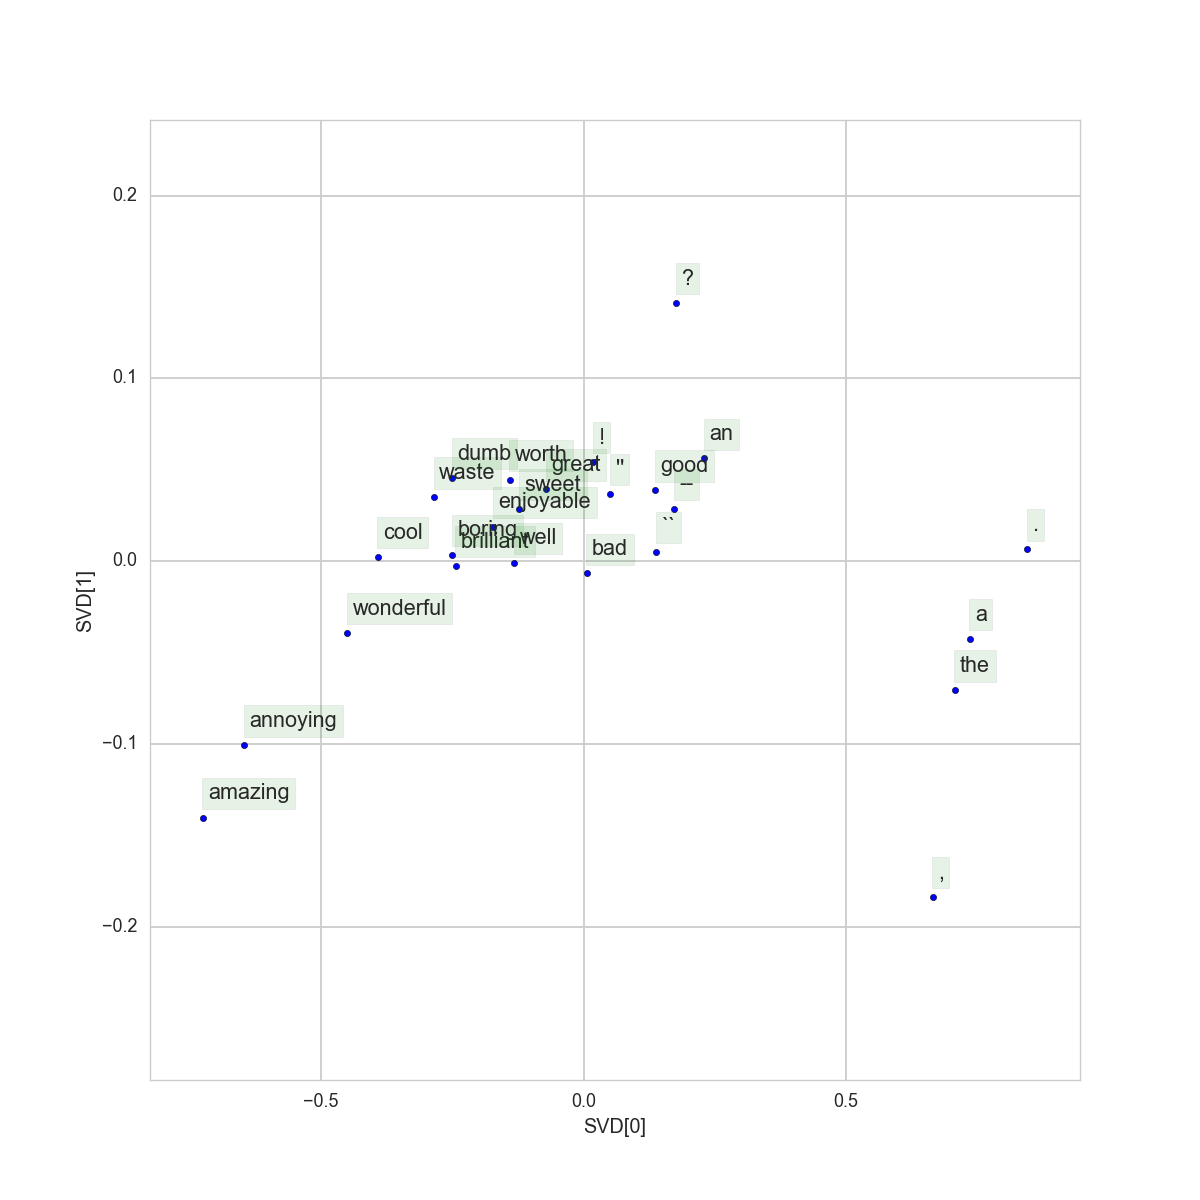
\includegraphics[scale=0.5]{../q3_word_vectors.png}
\caption{Plot of the first two components of 10 dimensional $\cal{R}^{\texttt{n}}$ word embedding for the \textbf{SST}. The words \texttt{a}, \texttt{the}, '\texttt{.}', '\texttt{,}' appear to have a distinct location away from the adjectives.}
\end{center}
\end{figure}

\clearpage
\myhwtitle{1}{3(h)}{\solutionsAuthor}
\bigskip
\noindent \textbf{Extra Credit} Implement the \texttt{CBOW} model in \texttt{q3\_word2vec.py}. \textbf{Note}: This part is optional but the gradient derivations for 
the \texttt{CBOW} in part (d) are not.
\vspace{5mm}

\noindent\rule{\textwidth}{0.4pt}\vspace{5mm}

\clearpage
\myrunninghwhead{1}{4 (Sentiment Analysis)}

\myhwtitle{1}{4}{\solutionsAuthor}
\bigskip
\noindent Now, with the word vectors you trained, we are going to perform a simple sentiment analysis. For each sentence in the Stanford Sentiment Treebank dataset, we are going to use the average of all the word vectors in that sentence as its feature, and try to predict the sentiment level of the said sentence. The sentiment level of the phrases are represented as real values in the original dataset, here we'll use five classes:
\begin{center}
\textbf{very negative}, \textbf{negative}, \textbf{neutral},\textbf{positive},\textbf{very positive}
\end{center}
which are represented by 0 to 4 in the code, respectively. For this part, you will learn to train a softmax regressor with SGD, and perform train/dev validation to imporve generalization of your regressor.
\clearpage

\myhwtitle{1}{4(a)}{\solutionsAuthor}

\bigskip
\noindent Implement a sentence featurizer and softmax regression. Fill in the implementation in \texttt{q4\_softmaxreg.py}. Sanity check your implementation with \texttt{python q4\_softmaxreg.py}.\vspace{5mm}

\noindent\rule{\textwidth}{0.4pt}\vspace{5mm}

\clearpage

\myhwtitle{1}{4(b)}{\solutionsAuthor}
\bigskip
\noindent Explain in fewer than three sentences why we want to introduce regularization when doing classification (in fact, most machine learning tasks).\vspace{5mm}

\noindent\rule{\textwidth}{0.4pt}\vspace{5mm}
Regularization helps prevent over-fitting. By limiting the parameter space it forces the model to have a higher chance of learning features (rather than memorizing the training data).
\clearpage

\myhwtitle{1}{4(c)}{\solutionsAuthor}

\bigskip
\noindent Fill in the hyperparameter selection code in \texttt{q4\_sentiment.py} to search for the `optimal' regularization parameter. \textbf{What values did you select? Report your train, dev, and test accuracies. Justify your hyperparameter search methodology in at most one sentence.}. \\

\noindent\textbf{Note:} you should be able to attain at least 30\% accuracy on dev.\vspace{5mm}

\noindent\rule{\textwidth}{0.4pt}\vspace{5mm}

\begin{table}[!h!p]
\begin{center}
\begin{tabular}{c c c}
\hline\hline
Reg & Train & Dev \\
\hline
0.00e+00 & 28.68 & 25.89 \\
1.00e-06 & 28.68 & 25.89 \\
2.14e-06 & 28.68 & 25.89 \\
4.57e-06 & 28.65 & 25.89 \\
9.77e-06 & 28.64 & 25.79 \\
2.09e-05 & 28.63 & 25.7 \\
4.47e-05 & 28.65 & 25.89 \\
9.55e-05 & 28.5 & 26.07 \\
2.04e-04 & 28.04 & 26.16 \\
4.37e-04 & 27.43 & 25.43 \\
9.33e-04 & 27.22 & 25.43 \\
2.00e-03 & 27.22 & 25.52 \\
4.27e-03 & 27.24 & 25.52 \\
9.12e-03 & 27.25 & 25.52 \\
1.95e-02 & 27.25 & 25.52 \\
4.17e-02 & 27.25 & 25.52 \\
8.91e-02 & 27.25 & 25.52 \\
1.91e-01 & 27.25 & 25.52 \\
4.07e-01 & 27.25 & 25.52 \\
8.71e-01 & 27.25 & 25.52 \\
1.86e+00 & 27.25 & 25.52 \\
3.98e+00 & 27.25 & 25.52 \\
\hline\hline
\end{tabular}
\end{center}
\end{table}
% Reg   Train   Dev
% 0.000000E+00  28.745318 27.066303
% 1.000000E-05  28.710206 26.612171
% 1.383648E-05  28.698502 26.793824
% 1.914482E-05  28.628277 26.702997
% 2.648969E-05  28.639981 26.793824
% 3.665241E-05  28.651685 26.793824
% 5.071404E-05  28.663390 27.066303
% 7.017038E-05  28.757022 26.975477
% 9.709111E-05  28.850655 26.612171
% 1.343399E-04  28.827247 26.612171
% 1.858792E-04  28.370787 25.703906
% 2.571914E-04  28.019663 25.522252
% 3.558624E-04  27.610019 25.794732
% 4.923883E-04  27.364232 25.613079
% 6.812921E-04  27.247191 25.249773
% 9.426685E-04  27.223783 25.340599
% 1.304321E-03  27.235487 25.431426
% 1.804722E-03  27.223783 25.431426
% 2.497100E-03  27.235487 25.522252
% 3.455107E-03  27.235487 25.522252
% 4.780653E-03  27.235487 25.522252
% 6.614741E-03  27.247191 25.522252
% 9.152473E-03  27.247191 25.522252
% 1.266380E-02  27.247191 25.522252
% 1.752224E-02  27.247191 25.522252
% 2.424462E-02  27.247191 25.522252
% 3.354602E-02  27.247191 25.522252
% 4.641589E-02  27.247191 25.522252
% 6.422325E-02  27.247191 25.522252
% 8.886238E-02  27.247191 25.522252
% 1.229543E-01  27.247191 25.522252
% 1.701254E-01  27.247191 25.522252
% 2.353937E-01  27.247191 25.522252
% 3.257021E-01  27.247191 25.522252
% 4.506570E-01  27.247191 25.522252
% 6.235507E-01  27.247191 25.522252
% 8.627748E-01  27.247191 25.522252
% 1.193777E+00  27.247191 25.522252
% 1.651767E+00  27.247191 25.522252
% 2.285464E+00  27.247191 25.522252
% 3.162278E+00  12.816011 12.806540

% Best regularization value: 0.000000E+00
% Test accuracy (%): 26.289593

\clearpage

\myhwtitle{1}{4(d)}{\solutionsAuthor}

\bigskip
\noindent Plot the classification accuracy on the train and dev set with respect to the regularization value, using a logarithmic scale on the x-axis. This should have been done automatically. \textbf{Include \texttt{q4\_reg\_acc.png} in your homework write up.} Briefly explain in at most three sentences what you see in the plot.\vspace{5mm}

\noindent\rule{\textwidth}{0.4pt}\vspace{5mm}

\begin{figure}[!h!p]
\begin{center}
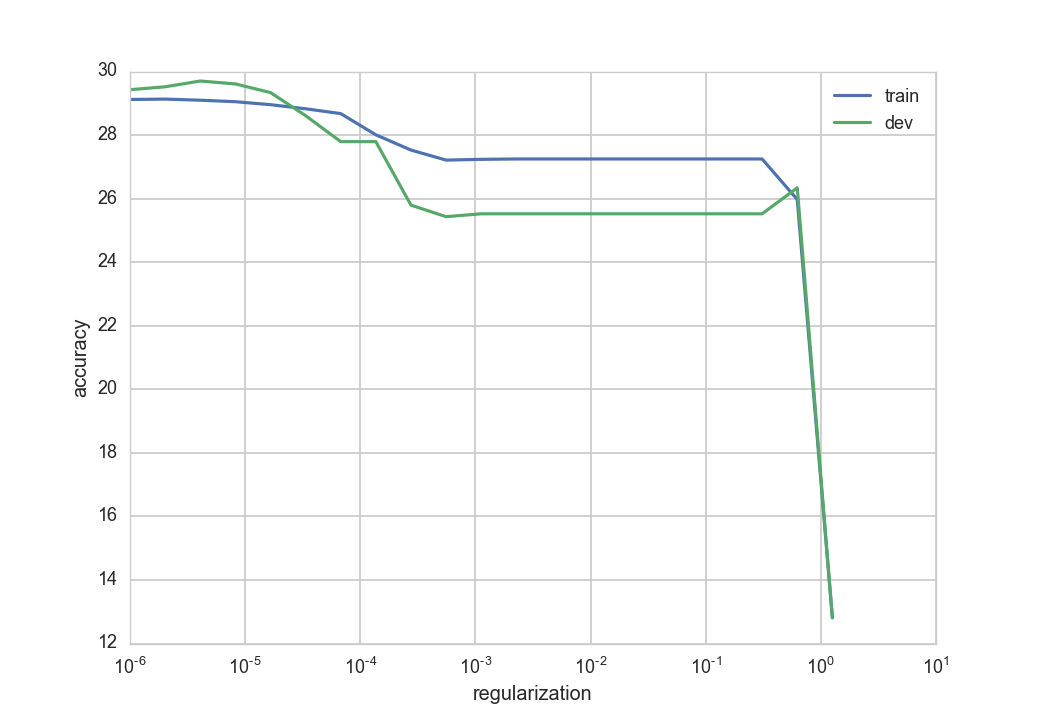
\includegraphics[scale=0.5]{../q4_reg_v_acc.png}
\end{center}
\end{figure}


%%%% End solution and document %%%%%%%%%%%%%%%%%%%%%%%%%%%%%%%%%%%%
\end{document}